\documentclass[final]{cvpr}

\usepackage{times}
\usepackage{epsfig}
\usepackage{graphicx}
\usepackage{amsmath}
\usepackage{amssymb}

% Include other packages here, before hyperref.
\usepackage{acro}
\usepackage{csquotes}
\usepackage{mathtools}
\usepackage[ruled]{algorithm2e}

% If you comment hyperref and then uncomment it, you should delete
% egpaper.aux before re-running latex.  (Or just hit 'q' on the first latex
% run, let it finish, and you should be clear).
\usepackage[pagebackref=true,breaklinks=true,colorlinks,bookmarks=false]{hyperref}


\def\cvprPaperID{****} % *** Enter the CVPR Paper ID here
\def\confYear{2021}

\newcommand{\q}[1]{\enquote{#1}}
\newcommand{\Par}[1]{\left(#1\right)}
\newcommand{\Brac}[1]{\left[#1\right]}
\newcommand{\Set}[1]{\left\{#1\right\}}
\DeclarePairedDelimiter{\abs}{|}{|}
\DeclarePairedDelimiter{\norm}{\lVert}{\rVert}

\newcommand{\acdef}[2]{
	\DeclareAcronym{#1}{
		short = #1,
		long = #2,
	}
}
\acdef{RMSE}{root mean squared error}
\acdef{KNN}{$k$-nearest neighbours}
\acdef{SVD}{singular value decomposition}
\acdef{NCF}{neural collaborative filtering}
\acdef{CF}{collaborative filtering}
\acdef{SGD}{stochastic gradient descent}


\begin{document}

\title{
	Project report \\~\\
	\large{Team name: M2 Robo}
}

\author{
	Lee Chun Yin\\
	3035469140\\
	\and
	Chiu Yu Ying\\
	3035477630
	\and
	Chan Kwan Yin\\
	3035466978 \\
	Team leader
}

\maketitle

\clearpage

\section{Introduction}
\subsection{\ac{CF}}
\ac{CF} is a technique for recommendation system,
in which historical feedback data are used to infer connections between users and products~\cite{FactorMeet}.
While additional features can be introduced to offset certain bias effects~\cite{BellKor2008},
two inputs (user and product) and one output (user rating on the product) are generally sufficient
to train a \ac{CF} model without involving domain-specific data.

Two major approaches for \ac{CF} include neighbourhood models and latent factor models.
Neighbourhood models compare the similarity between users
and recommend products positively rated by similar users,
while latent factor models perform dimensional reduction on both users and movies
to a common, smaller set of feature attributes such that
users are recommended with movies of more coherent features.

\subsection{The Netflix Prize dataset}
The Netflix Prize is a competition for the prediction of users' favour of movies.
The dataset provides existing ratings of users on given movies,
and models are trained to predict new ratings.

\subsubsection{Dataset format}

The dataset contains 100480507 rows of data structured in the following format:

\begin{tabular}{|c|c|c|c|}
	\hline
	User ID & 490189 discrete values \\ \hline
	Movie ID & 17770 discrete values \\ \hline
	Rating & 1, 2, 3, 4, 5 \\ \hline
	Date & Dates from 1999 to 2005 \\ \hline
\end{tabular}

\subsubsection{Distribution of ratings}
Ratings are mostly distributed around 3 and 4,
as shown in Figure \ref{fig:rating-freq}.

Except for some extreme cases, the number of ratings per user over the 7 years
mostly follow an exponential relation for users from 10 to 1000 ratings,
as shown in Figure \ref{fig:user-rating-freq}.
The top 10 users with the highest number of ratings
range from 17651 to 8877.

For movies with at least 100 ratings (which is the case for the majority),
their numbers of ratings demonstrate a similar but more concave relationship,
as shown in Figure \ref{fig:movie-rating-freq}.

\begin{figure}
	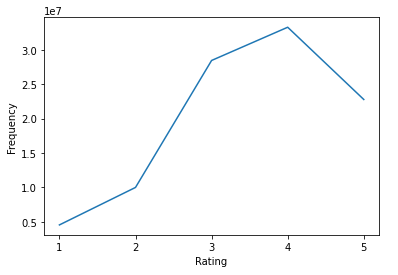
\includegraphics[width=0.5\textwidth]{screenshot20210422222105.png}
	\caption{Frequency of ratings}
	\label{fig:rating-freq}
\end{figure}

\begin{figure}
	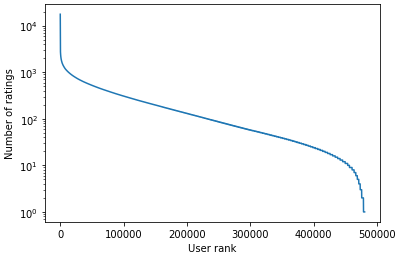
\includegraphics[width=0.5\textwidth]{screenshot20210422222340.png}
	\caption{Number of ratings per user}
	\label{fig:user-rating-freq}
\end{figure}

\begin{figure}
	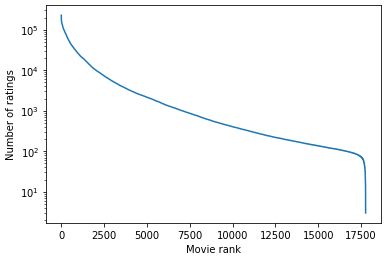
\includegraphics[width=0.5\textwidth]{screenshot20210422223229.png}
	\caption{Number of ratings per movie}
	\label{fig:movie-rating-freq}
\end{figure}

\subsubsection{Evaluation process}
To evaluate performance, 1425333 rows (about 1.42\% of all data) are specified as the standard "probe".
We perform analysis in the following procedure:

\begin{enumerate}
	\item Train the model with the 99055174 non-probe rows.
	\item Predict user ratings with the 1425333 probe rows.
	\item Compute the \ac{RMSE} between the predicted data and actual data.
    $$ \text{RMSE} = \sqrt{\sum_{(i, j) \in E} \frac{{(\hat r_{ij} - r_{ij})}^2}{\left| E \right|}} $$
where $E$ is the set of retained evaluation data.
\end{enumerate}


In this project, we evaluate three models, namely:

\begin{itemize}
	\item \ac{KNN}, a simple neighbourhood model
	\item \ac{SVD}, a latent factor model that accounts for user bias
	\item \ac{NCF}, a latent factor model that represents features with neural network weights
\end{itemize}

Originally, we proposed three models KNN, SVD and SVD++ (a SVD model with time features).
Due to the high similarity between SVD and SVD++,
we proposed the use of NCF instead,
while the additional time effect bias in SVD++ is left out as a to-do.

\subsection{Notations}
In this report, we denote variables about the dataset as follows:
\begin{itemize}
	\item $m$: number of users
	\item $n$: number of movies
	\item $N$: number of ratings
	\item $r_{ij}$: rating of user $i$ on movie $j$
	\item $\varepsilon_{ij}$: prediction error $\hat r_{ij} - r_{ij}$
\end{itemize}

\section{Data preprocessing}
Due to performance issues with CSV parsing, we wrote a separate program \texttt{preprocess-dataset},
which reformats the input files into a numpy saved array
which contains the following columns derived from the original dataset:

\begin{itemize}
	\item User ID
	\item Movie ID
	\item Rating value
	\item Year of rating
	\item Day of year of rating
	\item Day of week of rating
	\item Whether the rating is probed data
\end{itemize}

The source code of \texttt{preprocess-dataset} can be found on our GitHub repo:
\url{https://github.com/SOF3/stat4609-project}

During runtime, the data are represented in \ac{CSR} format
for a sparse $m \times n$ matrix,
where the $i$th row represented user $i$ and the $j$th column represents movie $j$.
Although we originally planned to implement SVD++ using the three date-related columns,
we eventually did not use them due to technical difficulties with bias interpolation over time.

\section{\ac{KNN}}
\ac{KNN} is an example of neighbourhood models.
It seeks to provide recommendations based on the behaviour of similar users.
In \ac{KNN} model, we assume that similar users will give close ratings on similar movies.
To predict the rating $\hat r_{ij}$ of user $i$ on movie $j$ ($1 \le i \le m, 2 \le j \le n$),
the $k$ most similar users ($n_1, \ldots, n_k$) to user $i$ are computed based on similar choices of ratings,
and $\hat r_{ij}$ is estimated based on the known values $r_{n_1j}, \ldots, r_{n_kj}$.

\subsection{Algorithm}
The training algorithm involves the following steps:

The algorithm first finds $q$, the set of $q$ users with the highest number of ratings.
The distance $d(i, j)$ for $i \in [1, m], j \in q \setminus \Set{i}$ is then computed,
and the neighbourhood $K_i \subset q$ of each user $i$ is evaluated as the $k$ users with the lowest distance.
The prediction of the rating $r_{ij}$ is computed by
aggregating the neighbourhood ratings with $A(\Set{r_{xj} : x \in K_i})$.
The memory complexity of these operations (except $d$ and $A$) is $O(qn)$.

In this KNN implementation, there are four hyperparameters to be considered, namely neighbourhood size $k$, neighbourhood candidate size $q$, distance function $d$ and aggregation function $A$.

\subsubsection{Neighbourhood size $k$}
$k$ refers to the number of nearest neighbours to be included in recommendation system. 

A large value of $k$ would reduce accuracy as users with lower similarity are selected.
On the other hand, a small value of $k$ would be biased over the choice of the most similar user.
We have tested with different values of $k$ with different values of the other hyperparameters.

As a baseline model, we also set $k=m$, i.e.
to evaluate the RMSE by taking the plain arithmetic mean of all users.

\subsubsection{Neighbourhood candidate size $q$}
$q$ means the number of neighbour candidate the recommendation system considered. 
We tried different values of $q$, which led to different sets of k-nearest neighbours being selected each time.

\subsubsection{Distance function $d$}
The distance function $d: \mathbb R^n \times \mathbb R^n \to [0, 1]$
observes the deviation in interests between two different users.
$d(i, j) = 0$ iff $i = j$, and $d(i, j) = d(j, i) \forall i = j$.
Although $d(i, j) < d(i, k)$ implies that $j$ is more similar to $i$ than $k$ is,
it is not necessary that $d$ follows triangular inequality.

\paragraph{Cosine}
The cosine distance is defined as
$$ d(\mathbf x, \mathbf y) = 2 \frac
{\Par{\mathbf x - \mathbf b} \cdot \Par{\mathbf y - \mathbf b}}
{\norm{\mathbf x - \mathbf b} \norm{\mathbf y - \mathbf b}} - 1 $$
where $\mathbf b = \frac1n \sum_{i=1}^m \mathbf r_{i\cdot}$,
i.e. the mean rating of each movie.
This metric emphasizes the difference between users who gave ratings better or worse than the average,
e.g. the difference between $3$ and $5$ is more important than the difference between $1$ and $3$
when the average rating is $4$.
It can be thought of a metric to determine how "abnormal" a user is.
The multiplier is to correct the distance range to $[0, 1]$.

\paragraph{$p$-norm}
The $p$-norm distance is defined as the $p$-norm of two vectors
normalized by the maximum possible distance, i.e.
$$ d(\mathbf x, \mathbf y) = \frac
{\Par{\sum_{i=1}^n \abs{x_i - y_i}^p}^{1/p}}
{4 n^{1/p}} $$.

\subsubsection{Aggregation function $A$}
We computed both baseline and average aggregation functions.

\subsection{Findings}

\subsubsection{Baseline model result}
The RMSE value attained in baseline model is $1.0528$.


\subsubsection{Cosine distance model result}
\begin{figure}[h]
	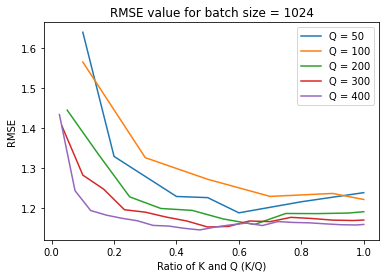
\includegraphics[width=0.5\textwidth]{knn-cosine-graph.png}
	\caption{RMSE for different combination of  q and k with cosine distance function}
	\label{fig:rmse-knn-QK}
\end{figure}

We can see the RMSE values decreased with the increasing $q$ value in general.
The curve with $q = 400$ has the smallest values for nearly all ratio of $k$ and $q$.
The curve with $q = 50$ however has larger values for most of the ratio values than the curve with $q = 100$.
All the curves have non-smooth logarithmic curves with fluctuations between ratio = 0.1 to ratio = around 0.7. 
The lowest RMSE value attained with the cosine distance function is $1.1455$ with ratio = 0.475 ($q = 400$ and $k=190$).
For the other values of $q$, when $q = 300$, the lowest value found in ratio = 0.5 ($k = 150$).
When $q = 200$, the lowest value belonged to ratio = 0.65 ($k = 130$).
When $q = 100$, the lowest value attained at ratio = 1 ($k = 100$).
When $q = 50$, the lowest belonged to ratio = 0.6 ($k = 30$).
To conclude, the ratios for the lowest value of RMSE for each curves varied.

\subsubsection{$p$-norm}
We tested $1$-norm (taxicab) and $2$-norm (Euclidean) with smaller data sizes
and discovered that they have significantly worse results (RMSE $1.176, 1.174$)
compared to cosine metric with the same dataset (RMSE $1.106$).

Since the computation of $p$-norm requires allocating a tensor of $nqb$ integers
(where $b$ is the batch size), which implies a large memory size is required.
A smaller choice of $b$ must be selected, which greatly reduces the speed of model training.
Considering the unsatisfactory RMSE of $p$-norm under smaller data sizes,
we do not evaluate them for the full dataset.

\section{\ac{SVD}}
\subsection{Background}
SVD assumes that ratings are modelled with the following formula:

$$ r_{ij} = \mu + a_i + b_j + \sum_{x=1}^k u_{ix} v_{jx} + \varepsilon
\text{ for } i \in [1, m], j \in [1, n] $$

$\mu$ is the global baseline score.
$a_i$ and $b_j$ are the user and movie bias,
which assumes that users and movies tend to have their own drift from the baseline ratings.
In terms of psychology, this can be interpreted as
certain users with more conservative with their ratings
or certain movies that result in poor impression.
These user/movie bias values are global to all movies/users,
so the model separates them from the latent factors.
The model also assumes that movies can be assessed with up to $k$ metrics,
which users have various interests about.
This is represented by the latent factors $u_{ix}$ and $v_{jx}$.

The algorithm computes $\mu$ as the mean of all ratings $\frac1{mn} \sum_{i,j} r_{ij}$,
and the bias values as user and movie rating means
$\frac1n \sum_j (r_{ij} - \mu), \frac1m \sum_i (r_{ij} - \mu)$.
The latent factors are initialized with the distribution $\operatorname N(0, \frac\sigma{200})$,
where $\sigma$ is the standard deviation of all ratings
and $200$ is an arbitrarily selected number based on actual trials.
This ratio is not exposed as a hyperparameter since descent parameters are random.
The reason for using a normal distribution instead of a constant value is that
the gradient descent formula suffers from division by zero
if the parameters are initialized as zero.

The gradient descent formula is derived to be

$$ \begin{cases}
	u_{ik} &\leftarrow u_{ik} + \alpha \Par{ \sqrt{s_i} \varepsilon_{ij} v_{jk} - \lambda u_{ik} } \\
	v_{jk} &\leftarrow v_{jk} + \alpha \Par{ \sqrt{s_j} \varepsilon_{ij} u_{ik} - \lambda v_{jk} }
\end{cases} $$

where $s_i, s_j$ are the number of ratings for the user/movie.

\subsubsection{Learning rate $\alpha$}
The learning rate determines the amount of gradient descent to apply in each epoch.
Since each user/movie has very different number of ratings, the descent in each iteration
is divided by the square root of the number of ratings.
As such, the learning rates selected are slightly higher than usual.

\subsubsection{Regularization $\lambda$}
Regularization is applied to avoid overfitting in the model.
It subtracts the descent with a proportion of the original latent factors.

\subsubsection{Rank of factorization $k$}
The model assumes that movies and user interests are matched using a discrete number of metrics.
This is modelled using different ranks of factorization.
It is expected that each rank represents some linear combination of the actual metrics.
A small choice of $K$ limits the best possible accuracy of the model,
while a large choice of $k$ tends to cause overfitting.
In fact, in preliminary tests with $m=10000, n=1000$,
we discovered that choosing $k=100$ brought excellent train accuracy but very poor test RMSE.

\subsubsection{Number of epochs $\xi$}
In each epoch, all training data are cycled through once
and the total training RMSE is reported.

Due to time constraints, we only train up to $\xi=15$ or $\xi=20$ for each model.
However, it was tested on smaller tests that
an infinite number of epochs shall converge in RMSE.

\subsubsection{Batch size $\beta$}
Due to performance reasons, $\varepsilon_{ij}$ is recomputed in batches
(as an instance of minibatch stochastic gradient descent).
The batch size is selected as $1048576$ for all models evaluated.

\subsection{Findings}
For all models, we set $\beta=1048576$ and $\xi=20$,
except for the model with $k=15$, we set $\xi=15$ to reduce training time,
and for the model with $\alpha=0.2$, we terminated the model early at $\xi=7$
as the RMSE turned out to diverge to infinity.

We evaluated the effects of $\alpha$, $\lambda$ and $k$ and obtained the following results.
We denote $e_\xi^{(t)}$ as the train RMSE at epoch $\xi$
and $e_\xi^{(p)}$ as the test RMSE at epoch $\xi$.

\hspace{-0.5cm}
\begin{tabular}{|c|c|c|c|c|c|c|}
	\hline
	$\alpha$ & $\lambda$ & $k$ & $e_{15}^{(t)}$ & $\xi$ & $e_\xi^{(t)}$ & $e_\xi^{(p)}$
	\\ \hline
	$0.05$ & $0$ & $10$ & $0.88432$ & $20$ & $0.84926$ & $0.95728$
	\\ \hline
	$0.05$ & $0.01$ & $10$ & $0.88440$ & $20$ & $0.84937$ & $0.95726$
	\\ \hline
	$0.05$ & $0.05$ & $10$ & $0.88474$ & $20$ & $0.84985$ & $0.95718$
	\\ \hline
	$0.2$ & $0.01$ & $10$ & N/A & $7$ & $44.040$ & $91.534$
	\\ \hline
	$0.05$ & $0.01$ & $20$ & $0.87771$ & $15$ & $0.87771$ & $0.96909$
	\\ \hline
\end{tabular}

\vspace{1cm}

The RMSE plots of the models are shown in order below.

\begin{figure}[h]
	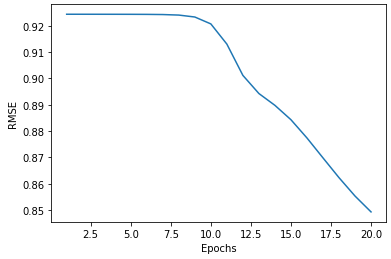
\includegraphics[width=0.5\textwidth]{screenshot20210504225232.png}
	\caption{SVD, $\lambda=0$}
\end{figure}

\begin{figure}[h]
	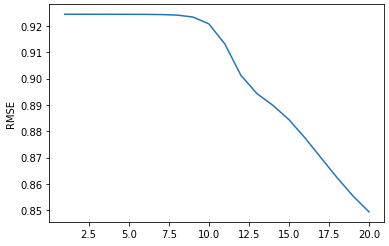
\includegraphics[width=0.5\textwidth]{screenshot20210504225440.png}
	\caption{SVD baseline, $\alpha=0.05, \lambda=0.01, k=10$}
\end{figure}

\begin{figure}[h]
	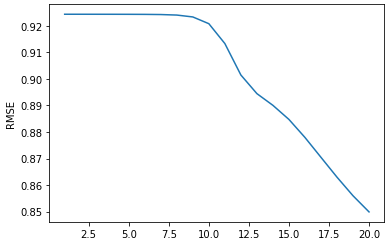
\includegraphics[width=0.5\textwidth]{screenshot20210504225504.png}
	\caption{SVD, $\lambda=0.05$}
\end{figure}

\begin{figure}[h]
	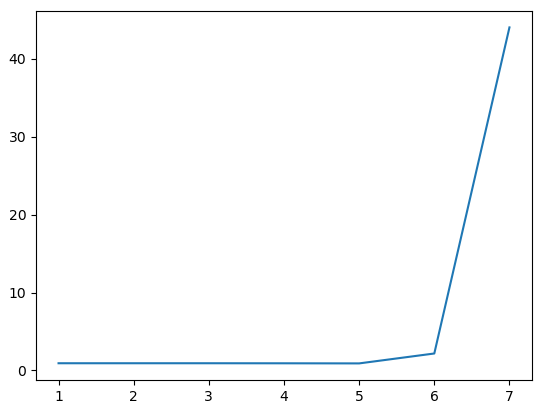
\includegraphics[width=0.5\textwidth]{screenshot20210504225138.png}
	\caption{SVD, $\alpha=0.2$}
\end{figure}

\begin{figure}[h]
	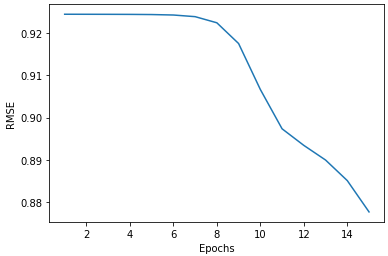
\includegraphics[width=0.5\textwidth]{screenshot20210504230954.png}
	\caption{SVD, $k=20$}
\end{figure}

The results show that $\lambda$ worsens the train RMSE but improves the test RMSE.
This is visualized by the inverse relation between train RMSE and test RMSE
in Figure \ref{fig:svd-train-test-lambda}.

Although the train RMSE converges very slowly at first,
it appears to have increasing rate of convergence
in each of the converging plots,
and it is expected that they will continue converging
based to preliminary tests with a smaller dataset.
On the other hand, although setting a larger learning rate
appeared to increase the initial rate for train RMSE reduction,
the RMSE suddenly increases up to $2$ and then $40$ at the $5$th epoch.
To study this issue, we plotted a histogram of the latent factors across epochs
based on a smaller dataset, and we obtained the result in Figure \ref{fig:svd-histogram}.
It appears that the latent factors tend to diverge to large values
(which we clipped into the range $[-5, 5]$ to avoid getting useless infinite values)
as $\xi$ increases.
In other words, a large choice of $\alpha$ leads to a catastrophic overshoot of gradient descent.

A higher choice of $k$ has also resulted in improved train RMSE.
However, the test RMSE is apparently worse than the other converging models with $k=10$,
even after discounting the effect of reduced $\xi$.

\begin{figure}[h]
	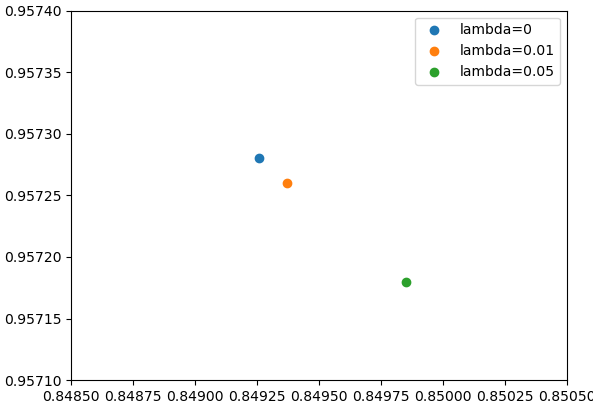
\includegraphics[width=0.5\textwidth]{screenshot20210504232929.png}
	\caption{SVD, $\lambda$ vs train RMSE vs test RMSE}
	\label{fig:svd-train-test-lambda}
\end{figure}

\begin{figure}[h]
	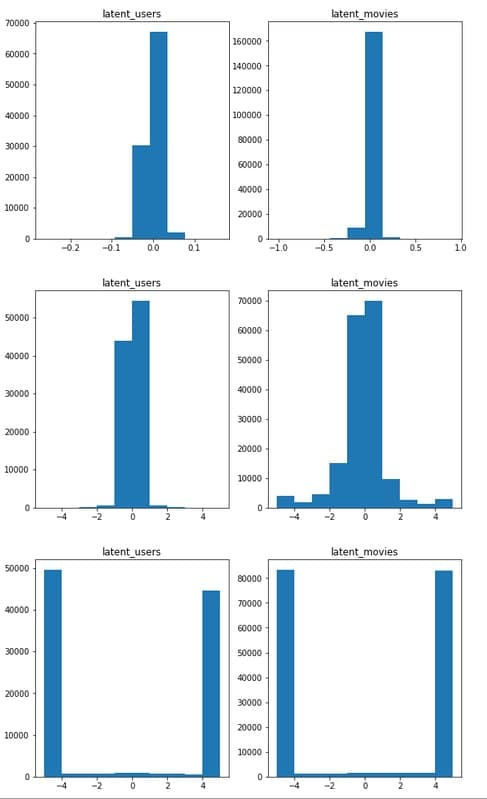
\includegraphics[width=0.5\textwidth]{svd-histogram.jpg}
	\caption{SVD, latent factor histogram}
	\label{fig:svd-histogram}
\end{figure}

\subsection{Future enhancement}
BellKor suggested that rating date has a bias effect on the rating value~\cite{BellKor2008}.
We plan to adopt this into the model so that
the exact bias effects can be visualized more clearly.

Further interpretation and analysis on the values trained in the model
would also be helpful in investigating the overfitting issue involved.
In particular, it would be useful to find the existence of
any complementary pairs of user-feature/movie-feature weights,
which imply the excess of the $k$ hyperparameter selection,
or singleton weights,
which imply direct memorization of a specific user/movie.

\section{\ac{NCF}}

Among all collaborative filtering techniques, matrix factorization (MF) become a standard approach to the model-based recommendation. Many research teams have put their efforts on enhancing it to break the accuracy record. 

However, it has several limitations such as the cold-start problem -- how the system provide recommendations to new users, how to recommend when new item is added without feature vector or embedding \cite{FMF}. Also, the use of dot product for recommending popular items will lead to the tendency of recommending popular items to those users without specific user interests. With the use of inner product of User and item feature embeddings, MF limits the capture of the complex relations  of the users and items interactions \cite{he2017neural}.

In this assignment, we aim to implement the new approach, Neural Collaborative Filtering (NCF), proposed by He team in 2017 \cite{he2017neural}. They suggested that their design of deep neural network can overcome the limitation of MF.

\subsection{Model structure}

This is the model proposed by He team in 2017 \cite{he2017neural}. Their proposed model uses a combination of matrix factorization and multi-layer perceptron techniques, and the hidden layers from the two techniques are combined by a fully-connected layer. However, their paper mainly focuses on the prediction of \textit{implicit user feedback}, that is, they are predicting the values of $y_{ui}$ where $y_{ui}=1$ when the observation (user $u$, item $i$) is observed, and $0$ when the
observation (user $u$, item $i$) is not observed. Thus, at the final stage of their proposed model, the output of the fully-connected layer is passed into a sigmoid function, such that the model only outputs values within $[0, 1]$. 

The problem of predicting implicit feedback is different from the problem we wish to solve in the Netflix dataset, because in the Netflix problem we wish to predict actual ratings from $[1, 5]$.
Nevertheless, we still think that He's paper provides a good starting point - We modify He's model by removing the final sigmoid function and changing the loss functions used directly, such that the neural network solves a regression problem instead of the original binary
classification problem.

The model proposed by He is split into 3 parts - Generalized Matrix Factorization, Multi-Layer Perceptron, and Neural matrix factorization. In fact, the third part is a combination of the previous two parts. For this part of our project, we will follow the same workflow as He and implement the 3 parts separately. 

\begin{figure}[h]
	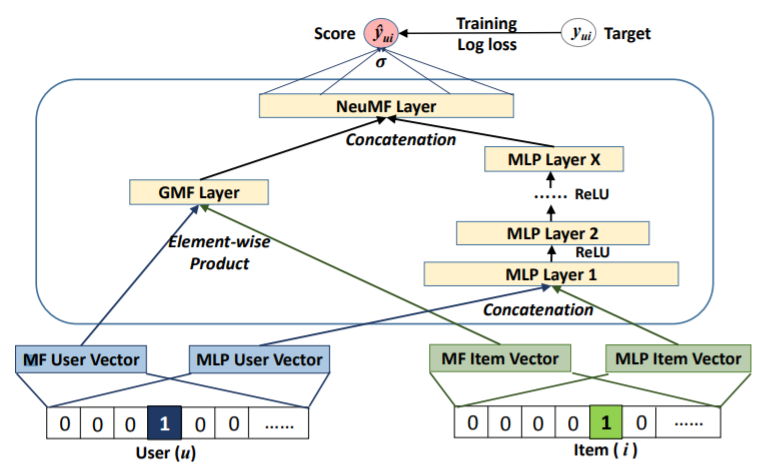
\includegraphics[width=0.5\textwidth]{./NeuCF.PNG}
	\caption{Neural Collaborative Filtering Model Design \cite{he2017neural}}
\end{figure}

\subsubsection{Model - Input Layer}

The input of the model are the user ID and item ID transformed to a binarized vector with one-hot encoding.

\subsubsection{Model - Embedding Layer}

For each user and each movie, we train two sets of embedding latent vectors. This is because one set of latent
vectors will be passed into the itemwise multiplication part
of the model (in He’s paper, it is called Generalized Matrix
Factorization (GMF)), and the other set of latent vectors will
be passed into the neural network part of the model (in He’s
paper, it is called Multi-Layer Perceptron (MLP)).

\subsubsection{Model - Generalized Matrix Factorization (GMF)}

In this part of the model, the user latent vector and item latent vector are combined via itemwise multiplication, similar to that in the SVD matrix factorization model. The output of this part is another vector with the same size at the latent vectors and is passed on to the final output layer of the model.

\subsubsection{Model - Multi-Layer Perceptron (MLP)}

In this part of the model, the user latent vector and item latent vector are first concatenated. Afterwards, the whole concatenated vector is passed through several layers of fully connected hidden linear layers, using the ReLU activation function. the output of this part is a vector depending on the output size of the last hidden layer and is passed on to the final output layer of the model.

\subsubsection{Model - Output Layer}

The final output layer takes in the vectors produced by the GMF and MLP parts of the model and concatenates them. The output of this part, which is the final output of the whole model, is a weighted sum of the vector elements, where the weights are model parameters to be learned. The final output layer produces a predicted score $\hat{y_{ui}}$.

\subsubsection{Model - Formula}
\bigskip
\textbf{ The formula of the GMF is as follow:}
$$\hat{y_{ij}} = f(P^T v_i Q^T v_j|P,Q,\Theta_f)$$

The variables with m users and n items are denoting as:
\begin{itemize}
    \item $P \in \mathbb{R}^{(m \times K)}$ latent factor matrix for users from embedding layer.
    \item $Q \in \mathbb{R} ^{(n \times K)}$ latent factor matrix for items from embedding layer.
    \item $f$ interaction function.    
    \item $\Theta_{f}$ model parameters of the interaction function $f$
\end{itemize}

\bigskip
\textbf{ For MLP $f$, it can be formulated as:}
$$f(P^T v_i, Q^T v_j) = \phi_{output}(\phi_X(...\phi_2(\phi_1(P^T v_i, Q^T v_j))...))$$

The mapping functions are as follow:
\begin{itemize}
    \item $\phi_{output}$: the mapping function for output layer
    \item $\phi_x$ the activation function for the $x$th hidden neural FC layer. $x$ is the number of the layers
\end{itemize}

\subsection{Technical Details}

The movies are loaded into a list with columns of Movie ID, User ID and Rating. Then, it will be fed into the test loader with batch size.

We select Adadelta as our optimizer. 
To have a better performance on the converge of loss function,we implement a scheduler with different combinations of hyperparameters of scheduler.

\subsection{Hyperparameters selection for scheduler}
There are two hyperparameters, namely
\begin{itemize}
    \item step size
    \item $\gamma$
\end{itemize}

\subsection{Hyperparameters selection for model}
In this MLP model, there are five hyperparameters to be selected, namely
\begin{itemize}
	\item Learning Rate ($\alpha$)
	\item Regularization ($\lambda$)
	\item Rank of factorization ($k$)
	\item Number of epoch ($x$)
	\item Batch Size ($N$)
\end{itemize}


\subsubsection{Learning Rate ($\alpha$)}
The learning rate indicates the speed at which the model learns. It controls how much to change the modal to respond the estimate error each time when the model weights are updated.

Rate with too small value may cause a long training time while a large value may allow the modal learning too fast to have less accurate or even not meaningful result.

\subsubsection{Rank of factorization ($k$)}
Intuitively, each rank represents some characteristic of a user or a movie. Users and movies that interact strongly on a rank would be affected.

A large value of $k$ increases the training time, memory consumption and probably the chance of overfitting,
while a low value of $k$ reduces the representativeness of the model and hence reduced accuracy.

\subsubsection{Number of epoch ($x$)}
The number of epochs defines the number of times that the modal will work through the whole training dataset.
Since we already report the training score for each epoch, it is adjusted to a value such that the training score appears to converge negligibly.

\subsubsection{Batch size ($N$)}
The batch size defines the number of samples to be passed through before the update of model parameters.

The small batch size usually can give a better performance since the model can start learning with a small subset and have more cycles to improve.

However, the smaller batch size costs the slower learning and hence more training time.

Taking these factors into consideration, we decided that the batch size $65535$ shall be used for all models, .

\subsection{Predictive test set score (RMSE)}
The model is evaluated by computing the RMSE between predicted and actual rating values:
$$ \text{RMSE} = \sqrt{\sum_{(i, j) \in E} \frac{{(\hat r_{ij} - r_{ij})}^2}{\left| E \right|}} $$
where $E$ is the set of retained evaluation data.


\subsection{Findings}

The following table exhaustively lists our test results. Train RMSE and Test RMSE refer to the RMSE value calculated for the training dataset and testing dataset respectively.

\hspace{-2cm}
\begin{tabular}{|c|c|c|c|c|c|c|c|}
	\hline
	Model & $k$ & $\alpha$ & $\gamma$ & Epochs & Train RMSE & Test RMSE
	\\ \hline
	GMF(1) & $100$ & $1$ & $0.7$ & $9$ & $1.07881$ & $1.08611$
	\\ \hline
	GMF(2) & $300$ & $1$ & $0.7$ & $9$ & $1.07930$ & $1.08696$
	\\ \hline
	GMF(3) & $100$ & $0.1$ & $0.9$ & $9$ & $1.07951$ & $1.08816$
	\\ \hline
	MLP(1) & $100$ & $1$ & $0.7$ & $8$ & $1.05487$ & $1.07873$
	\\ \hline
	MLP(2) & $300$ & $1$ & $0.7$ & $7$ & $1.03152$ & $1.11101$
	\\ \hline
	MLP(3) & $100$ & $0.1$ & $0.9$ & $7$ & $1.07000$ & $1.08372$
	\\ \hline
	NCF(1) & $100$ & $1$ & $0.7$ & $7$ & $1.05984$ & $1.08483$
	\\ \hline
	NCF(2) & $300$ & $1$ & $0.7$ & $7$ & $1.02703$ & $1.09038$
	\\ \hline
	NCF(3) & $100$ & $0.1$ & $0.9$ & $7$ & $1.06626$ & $1.08536$
	\\ \hline
\end{tabular}

\begin{figure}
	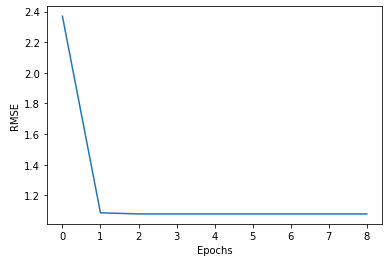
\includegraphics[width=0.5\textwidth]{screenshot20210415234153.png}
	\caption{RMSE graph for model GMF(1)}
\end{figure}

\begin{figure}
	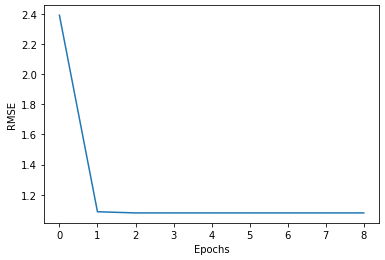
\includegraphics[width=0.5\textwidth]{screenshot20210415234346.png}
	\caption{RMSE graph for model GMF(2)}
\end{figure}

\begin{figure}
	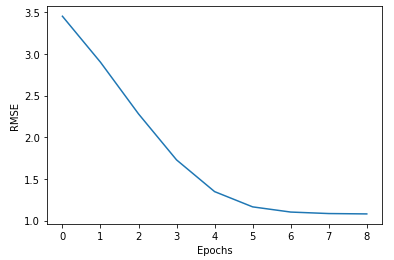
\includegraphics[width=0.5\textwidth]{screenshot20210415234450.png}
	\caption{RMSE graph for model GMF(3)}
\end{figure}

\begin{figure}
	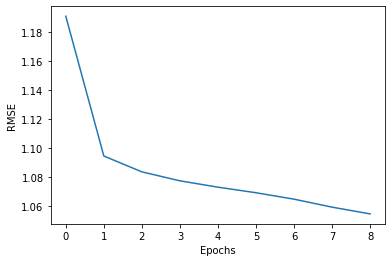
\includegraphics[width=0.5\textwidth]{mlp_1.png}
	\caption{RMSE graph for model MLP(1)}
\end{figure}

\begin{figure}
	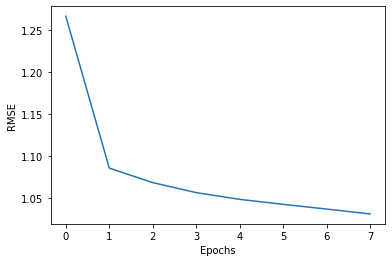
\includegraphics[width=0.5\textwidth]{mlp_2.png}
	\caption{RMSE graph for model MLP(2)}
\end{figure}

\begin{figure}
	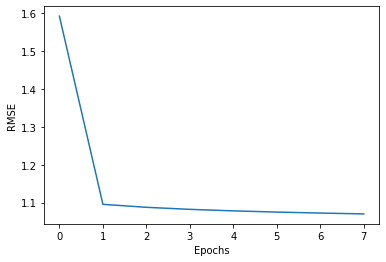
\includegraphics[width=0.5\textwidth]{mlp_3.png}
	\caption{RMSE graph for model MLP(3)}
\end{figure}

\begin{figure}
	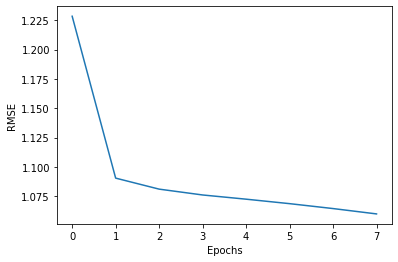
\includegraphics[width=0.5\textwidth]{ncf_1.png}
	\caption{RMSE graph for model NCF(1)}
\end{figure}

\begin{figure}
	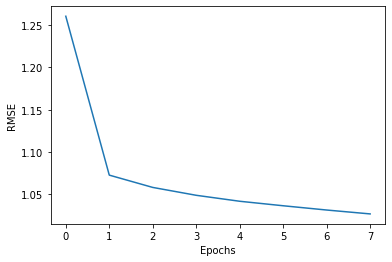
\includegraphics[width=0.5\textwidth]{ncf_2.png}
	\caption{RMSE graph for model NCF(2)}
\end{figure}

\begin{figure}
	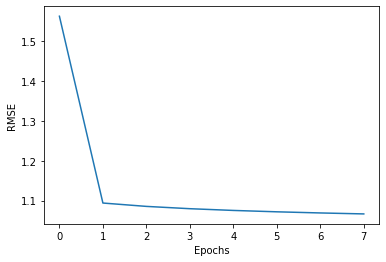
\includegraphics[width=0.5\textwidth]{ncf_3.png}
	\caption{RMSE graph for model NCF(3)}
\end{figure}

\hspace{10em}

For GMF, when comparing the results of tuning the value of rank from 100 to 300, we can see the RMSE curves have a similar shape in general. After epoch 0, both MSE values drop significantly by around 4.5 units and then the values remain constant. The shape becomes smoother than previous results by tuning learning rate to 0.1 and $\gamma$ to 0.9. 

For MLP, when raising the rank from 100 to 300, we observe that the train RMSE decreases but the test RMSE increases. This may be due to overfitting and that an embedding with length 300 is too much for the MLP model. The shapes of the training curves are similar, with a large drop after the epoch 0. The curve becomes less smooth and the loss increases after tuning the learning rate to 0.1 and $\gamma$ to 0.9.

For NCF, we have similar observations to the MLP model, that the increase in embedding size leads to increase in test RMSE. However, for embedding size of 300, the train and test RMSE are both lower than that of the MLP model. This may imply that more epochs are needed to train the NCF model as it has higher complexity. The training loss curves are similar to that of the MLP case. 

\section{Conclusion}

In our trained models, we find that the SVD model performs the best with RMSE test value 0.95718, possibly because of its simplicity. For the KNN, the best test RMSE value attained is 1.1455 with $q = 400$ and $k = 190$. In the NCF model, the best value attained is 1.07873 in MLP(1).

When training the models, we faced difficulties when dealing with the large dataset size of the Netflix dataset,
and we had to make adjustments to our model and training procedure.
For the KNN model, the original model we proposed constructs an $m \times n$ matrix to store all ratings which were too expensive in terms of memory usage,
and we had to use the "Top $Q$ optimization" technique proposed by Hong et al~\cite{Alpher01} instead.
For the SVD and NCF models, in order to finish model training within time constraints, we had to use optimization techniques such as vectorization, \ac{SGD} with minibatch optimization and adjusting batch size.
Further work can be extended upon this topic.
For example, it is noted that the RMSE value varies over different combinations of $k$ and $q$.
We believe that there is potential for KNN to further improve its performance by trying more combinations of the hyperparameters.
The importance of fine-tuning the hyperparameters also presented in the other two models (SVD and NCF) as well.
BellKor suggested that rating date has a bias effect on the rating value~\cite{BellKor2008}.
We plan to adopt this into the model so that
the exact bias effects can be visualized more clearly.
Further interpretation and analysis on the values trained in the model
would also be helpful in investigating the overfitting issue involved.
In particular, it would be useful to find the existence of
any complementary pairs of user-feature/movie-feature weights,
which imply the excess of the $k$ hyperparameter selection,
or singleton weights,
which imply direct memorization of a specific user/movie.

{\small
	\bibliographystyle{ieee_fullname}
	\bibliography{egbib}
}

\end{document}
